\documentclass{article}
\usepackage{graphicx} % Required for inserting images
\usepackage{subcaption}
\usepackage{amsmath, amssymb, booktabs}
\usepackage{hyperref}
\usepackage{comment}
\usepackage{xcolor}  % Required for color customization
\hypersetup{
  colorlinks=true,  % Activates colored links
  linkcolor=blue,   % Color of internal links (section*s, pages, etc.)
  citecolor=blue,   % Color of citation links
  urlcolor=blue     % Color of external links (URLs)
}
\graphicspath{ {./figures/} }


\title{Classless Classification: \\
\large Raisin Classification with K-means model}
\author{Jonathan Ferdinand, Devina Gera, Archimedes Li, Henry Liu, \\Katherine Shi, Sam Stevens}
\date{\today}

\begin{document}

\maketitle

\section*{Introduction}

We use and compare two different classification models, k-nearest neighbors and decision trees.  Each model is tasked with classifying raisins into the Kecimen or Besni class based on a set of 7 independent variables (see Data Description).

\vspace{5mm}

\noindent The k-nearest neighbors (kNN) model works by finding the k closest data points using Euclidean distance, and selects the most common class among those neighbors.  Some assumptions for the kNN to work well is that all features are normalized, and that there are no unnecessary features.  Some benefits to the kNN model is that it is non-parametric, which makes it flexible to different data distributions.  However, it has a major drawback with computational cost, since it needs to calculate the distance with every single point for each prediction.

\vspace{5mm}

\noindent The decision tree model recursively splits the data according to a threshold of a variable.  Because every decision is explicitly listed and the decision tree can be clearly graphically visualized, the decision tree has a high interpretability.  They are also robust to extraneous features and outliers, thus no data assumptions are necessary.  However, decision trees are prone to overfitting, so it is important to limit the number of branches through methods like pruning.


\section*{Data Description}
Our dataset consisted of 900 instances, each pertaining to an image of a raisin. The dataset extracted 7 features (listed below) from each of the images, along with a label of either Kecimen or Besni, which are the raisin types (and the label that we classified between). There were 450 instances for each label.

\begin{enumerate}
    \item Area - Gives the number of pixels within the boundaries of the raisin.
\item Major axis length - Gives the pixel length of the main axis, which is the longest line that can be drawn on the raisin.

\item Minor axis length - Gives the pixel length of the small axis, which is the shortest line that can be drawn on the raisin.

\item Eccentricity - It gives a measure of the eccentricity of the ellipse, which has the same moments as raisins.  Values closer to 0 indicate the raisin is more circular, and values closer to 1 indicate that the raisin is more elongated.

\item Convex area - Gives the number of pixels of the smallest convex shell of the region formed by the raisin.

\item Extent - Gives the ratio of the region formed by the raisin to the total pixels in the bounding box.  Ranges from 0 to 1.

\item Perimeter - It measures the environment by calculating the distance between the boundaries of the raisin and the pixels around it.

While looking through the data, we saw no obvious outliers, so we did not need to perform any form of data cleaning. 

Our data was found from Kaggle \cite{Raisin}. 

\end{enumerate}

\section*{Analysis}

We first shuffled the data to ensure raisin classes were well mixed rather than separated. We then split our data, using 70\% of the data for training and the remaining 30\% for testing. We also normalized the data between the ranges of 0 and 1 for the kNN model. 

\vspace{5mm}

\noindent We can see the diagonal plots for the model in figure \ref{fig:diagPlot}. There is a strong correlation between the AxisLengths, perimeter, and  Area, which makes sense. There is weak correlation between Extent and Area, Eccentricity and MinorAxisLength, (which is surprising considering that there is statistically significant correlation between eccentricity and MajorAxisLength), Extent and ConvexArea, Extent and MinorAxisLength. The remaining variables have some level of statistically significant correlation( refer to Fig \ref{fig:diagPlot} for more details).

\begin{figure}[h]
    \centering
    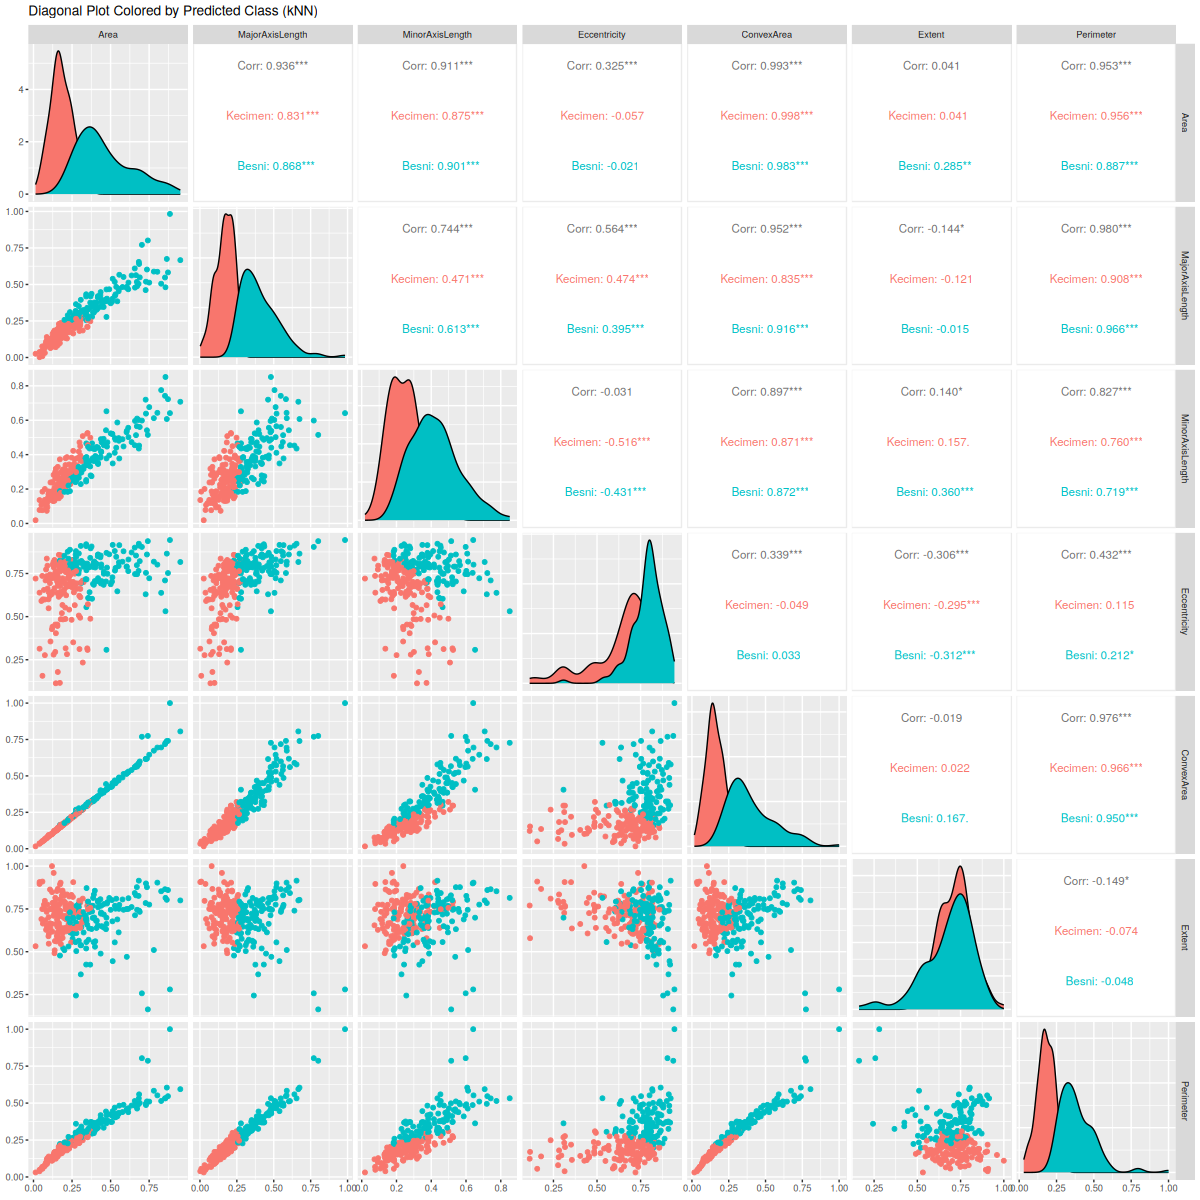
\includegraphics[width=1\linewidth]{knn_pairs_plot}
    \caption{Diagonal plots showing the correlation between all the combinations of predicting variables for the kNN model.}
    \label{fig:diagPlot}
\end{figure}

\vspace{5mm}

\noindent We used 10-fold cross-validation to find that $k = 41$ worked the best for our model with an accuracy of $86.7\%$. Figure \ref{fig:diagPlot} supports our assumption that certain features are grouped for different types of Raisin. The histograms along the diagonal show differing mean and standard deviation between the class of raisin and feature for all features other than extent and eccentricity. 


\clearpage

\section*{Model Evaluation}

\subsection*{kNN Model}
We ran our kNN model using subset selection.

\vspace{5mm}

\noindent To ensure optimality of features for using a kNN algorithm, we ran subset selection with 10-fold cross validation to determine the most impactful features.

\vspace{5mm}

\noindent We can see the output below.


\begin{verbatim}
 Variables Accuracy  Kappa AccuracySD KappaSD Selected
         1   0.7922 0.5844    0.04773 0.09547         
         2   0.8378 0.6756    0.04294 0.08587         
         3   0.8478 0.6956    0.03921 0.07843         
         4   0.8500 0.7000    0.04099 0.08198         
         5   0.8500 0.7000    0.03750 0.07499         
         6   0.8544 0.7089    0.03757 0.07514         
         7   0.8578 0.7156    0.03733 0.07466        *

\end{verbatim}

\noindent From the output, we saw that all predictor variables had similar impact on the final prediction, and after tests with various subsets, we determined that using all features for the kNN model was optimal.

\vspace{5mm}

\noindent We then used 10-fold cross-validation to find that the best k value is $k = 41$ with an accuracy of $86.7\%$ on the data with the following confusion matrix:

\begin{verbatim}
          Reference
Prediction Kecimen Besni
   Kecimen     119    27
   Besni         9   115
\end{verbatim}

\noindent Where $0$ pertains to Kecimen and $1$ is Besni. We can use these metrics to calculate the precision, recall, and F1-score of our model as well.

\vspace{5mm}

\noindent For the Kecimen class, we found

\begin{enumerate}
    \item Precision: 0.815

    \item Recall: 0.930

    \item F1-score: 0.869
\end{enumerate}

For the Besni class, we found

\begin{enumerate}
    \item Precision: 0.927

    \item Recall: 0.810

    \item F1-Score 0.865

\end{enumerate}

Overall, we see good performance from our kNN Model, with high precision, recall, F1-score, and accuracy.

The entire output can be found in Appendix B [\ref{sec:appendixB}], along with our code in Appendix A [\ref{sec:appendixA}].

\begin{figure}
	\centering
	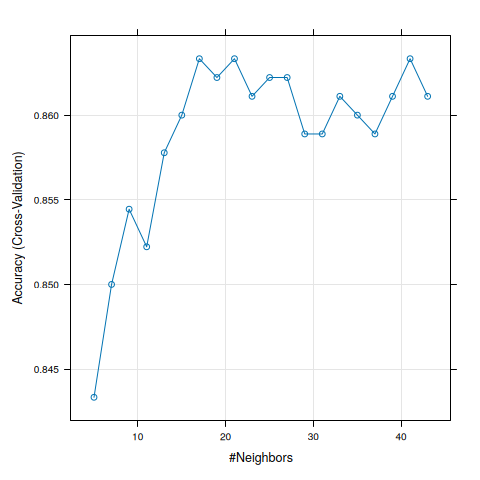
\includegraphics[width=\linewidth]{cv_plot}
	\caption{ Accuracy of our model as a function of number of neighbors during cross-validation.}
	\label{fig:cvPlot}
\end{figure}
\clearpage

\subsection*{Decision Tree Model}
We used 10-fold cross-validation again, to find the optimal tuning parameters, picking the model with the highest accuracy. The plot from the cross validation can be found in figure \ref{fig:tree_cv}

\noindent We trained our decision tree to find the split points shown in figure \ref{fig:tree_plot}.


\noindent Since decision trees are able to run on all features, we did not need to perform any subset selection.

\noindent We found the following confusion matrix on the test data.

\begin{verbatim}
         Actual
Predicted Kecimen Besni
        1     116    27
        2      12   115
\end{verbatim}

\noindent From the confusion matrix, we determined the accuracy to be 0.856.

\noindent Furthermore, we found the following metrics for precision, recall, and F1-score.

\noindent For the Kecimen class, we found

\begin{enumerate}
    \item Precision: 0.811

    \item Recall: 0.906

    \item F1-score: 0.856
\end{enumerate}

\noindent  For the Besni class, we found

\begin{enumerate}
    \item Precision: 0.906

    \item Recall: 0.810

    \item F1-Score: 0.855
\end{enumerate}

\subsection*{Comparison}

Overall, we found better accuracy using the knn model, as well as better precision, recall, and F1-score on average. This indicates that the knn model is more optimal for this dataset than the decision tree.

\begin{figure}[h]
    \centering
    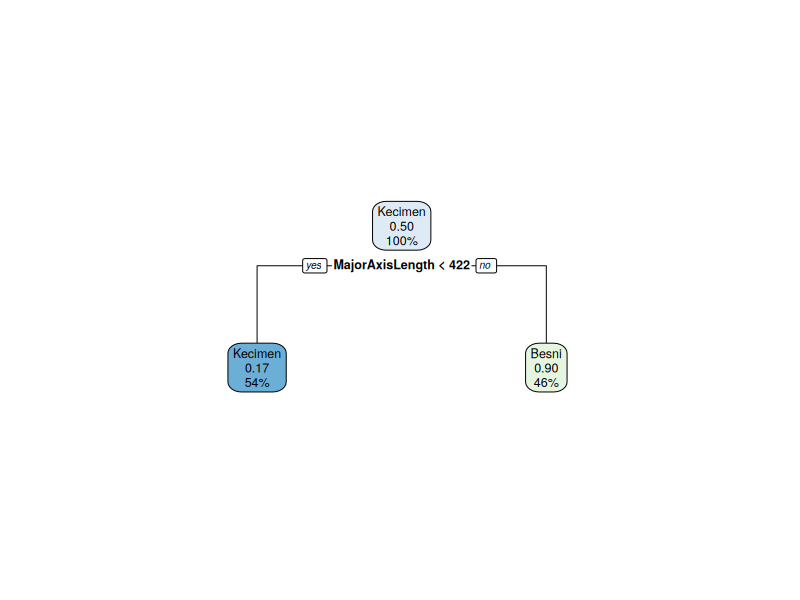
\includegraphics[width=.7\linewidth]{tree_plot}
    \caption{Diagram of decision choices at each level of trained decision tree}
    \label{fig:tree_plot}
\end{figure}
\begin{figure}[!h]
	\centering
	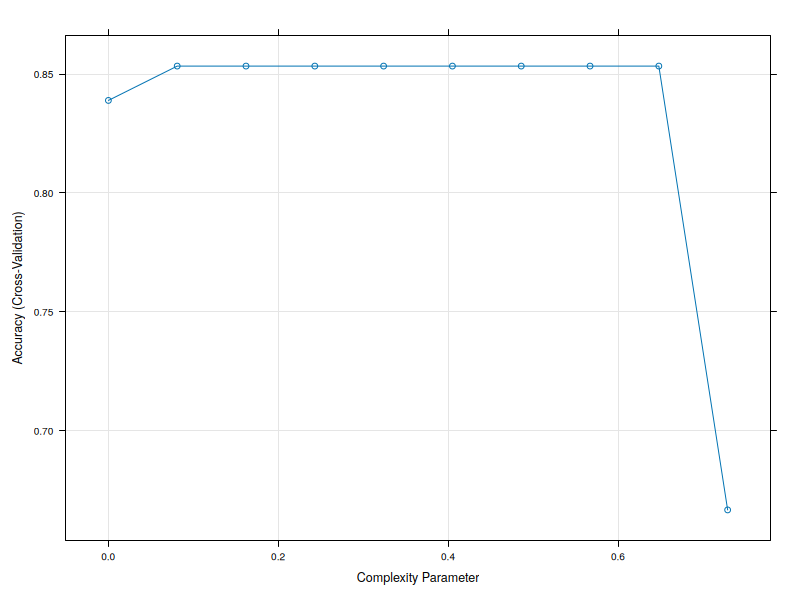
\includegraphics[width=\linewidth]{tree_cv_plot}
	\caption{Accuracy as a function of complexity parameter for the decision tree.}
	\label{fig:tree_cv}
\end{figure}


\clearpage
\section*{Conclusion}

Overall, we found good results with both the kNN model and the decision tree model. We saw slightly higher accuracy knn model, with 86.7\% accuracy, compared to 85.5\% using the decision tree. The robustness of both models and being able to take into account all features of the dataset likely led to good performance. In addition, we saw higher precision and recall metrics with the knn model as well, which may indicate that the data is not necessarily partitioned in space as well as we first thought.

\vspace{5mm}

\noindent Future steps may include testing with more robust models such as neural networks, or implementing ensemble methods such as random forests.

\begin{thebibliography}{9}

\bibitem{STHDA}
Lateef, Z. (2022, March 29). \emph{KNN Algorithm: A practical implementation of KNN algorithm in R.} Edureka. \url{https://www.edureka.co/blog/knn-algorithm-in-r/}

\bibitem{Raisin}
\emph{Raisin binary classification}. (2024, February 11). Kaggle. \url{https://www.kaggle.com/datasets/nimapourmoradi/raisin-binary-classification/data}


\bibitem{advert}
Blog, G. (2020, June 26). \emph{Best way to learn kNN Algorithm using R Programming}. Analytics Vidhya. \url{https://www.analyticsvidhya.com/blog/2015/08/learning-concept-knn-algorithms-programming/}

\newpage

\section*{Appendix A: Code}
\label{sec:appendixA}
The code is available \href{https://github.com/mshki/math-456/blob/main/essay_4/main.R}{on our github}, or below.

\begin{verbatim}
# Load required libraries
library("Cairo")
library("class")
library("caret")
library("rpart")
library("rpart.plot")
library("ggplot2")
library("tree")
library("randomForest")
library("GGally")

# --- Load and preprocess the data ---
raisins <- read.csv("data/Raisin_Dataset.csv")
raisins <- na.omit(raisins)  # Remove missing values

# Convert Class to binary: Besni = 1, Kecimen = 0
raisins$Class <- factor(raisins$Class, levels = c("Kecimen", "Besni"))
#raisins$Class <- ifelse(raisins$Class == "Besni", 1, 0)

# --- Normalize numeric features for KNN ---
normalize <- function(x) {
  return ((x - min(x)) / (max(x) - min(x)))
}
raisins_norm <- as.data.frame(lapply(raisins[1:7], normalize))
raisins_labels <- raisins$Class
raisins_norm$Class <- as.factor(raisins_labels)  # caret expects factors

# --- Feature selection using RFE (Recursive Feature Elimination) ---
set.seed(456)

# Define RFE control
rfe_ctrl <- rfeControl(functions = rfFuncs,  # Use random forest for ranking
                       method = "cv", 
                       number = 10)

# Run RFE
rfe_result <- rfe(x = raisins_norm[, 1:7],
                  y = raisins_norm$Class,
                  sizes = c(1:7),
                  rfeControl = rfe_ctrl)

# Show selected features
print(rfe_result)
selected_features <- predictors(rfe_result)
cat("Selected Features:", selected_features, "\n")

# --- Cross-validation to find the best K using caret ---
set.seed(11)
train_control <- trainControl(method = "cv", number = 10)  # 10-fold CV

# Train KNN model with internal CV
knn_cv_model <- train(Class ~ ., 
                      data = raisins_norm, 
                      method = "knn", 
                      trControl = train_control, 
                      tuneLength = 20)  # tries k = 1 to 20

# Output best model and k
print(knn_cv_model)
CairoPNG("figures/cv_plot.png")
plot(knn_cv_model)
dev.off()

# Get the best K value
best_k <- knn_cv_model$bestTune$k
cat("Best K:", best_k, "\n")

# --- Split dataset into train and test for evaluation using best K ---
set.seed(456)
train_idx <- sample(1:nrow(raisins), size = 0.7 * nrow(raisins))
train_data <- raisins_norm[train_idx, 1:7]  # only features
test_data  <- raisins_norm[-train_idx, 1:7]
train_labels <- raisins_norm$Class[train_idx]
test_labels  <- raisins_norm$Class[-train_idx]

# Predict with best K from cross-validation
knn_final_pred <- knn(train = train_data, test = test_data, cl = train_labels, k = best_k)

# --- Evaluate performance ---
confusionMatrix(knn_final_pred, test_labels, mode = "everything")

# --- Visualize predictions ---
plot_data <- test_data
plot_data$Predicted <- knn_final_pred
CairoPNG("figures/knn_pairs_plot.png", width = 1200, height = 1200)
ggpairs(plot_data, mapping = aes(color = Predicted),
        columns = 1:7, title = "Diagonal Plot Colored by Predicted Class (kNN)")
dev.off()

#  Decision Tree model for comparison ---
#raisins$Class <- factor(raisins$Class, levels = c(0, 1))
# --- Cross-validation for Decision Tree ---
set.seed(123)
tree_cv_model <- train(Class ~ ., 
                       data = raisins,
                       method = "rpart",
                       trControl = train_control,  # already defined as 10-fold CV
                       tuneLength = 10)  # explore different complexity parameters (cp)

# Output the best model and its complexity parameter
print(tree_cv_model)
CairoPNG("figures/tree_cv_plot.png", width = 800, height = 600)
plot(tree_cv_model)
dev.off()

# Use the best tree model to make predictions on the test set
tree_best_model <- tree_cv_model$finalModel

print("%%%%%% DECISION TREE %%%%%%")
CairoPNG("figures/tree_plot.png", width = 800, height = 600)
rpart.plot(tree_best_model)
dev.off()
tree_pred <- predict(tree_best_model, raisins[-train_idx,], type = "vector")
conf_matrix_tree <- table(Predicted = round(tree_pred), Actual = test_labels)
accuracy <- sum(diag(conf_matrix_tree))/sum(conf_matrix_tree)
print(conf_matrix_tree)
cat("Accuracy of Tree Model:", accuracy, "\n")
\end{verbatim}
\newpage
\section*{Appendix B: Code output}
\label{sec:appendixB}

\begin{verbatim}
Recursive feature selection

Outer resampling method: Cross-Validated (10 fold) 

Resampling performance over subset size:

 Variables Accuracy  Kappa AccuracySD KappaSD Selected
         1   0.7911 0.5822    0.06149  0.1230         
         2   0.8344 0.6689    0.06467  0.1293         
         3   0.8433 0.6867    0.05480  0.1096         
         4   0.8389 0.6778    0.05599  0.1120         
         5   0.8456 0.6911    0.05603  0.1121         
         6   0.8500 0.7000    0.06091  0.1218         
         7   0.8544 0.7089    0.06096  0.1219        *

The top 5 variables (out of 7):
   Perimeter, MajorAxisLength, Eccentricity, ConvexArea, Area

Selected Features: Perimeter MajorAxisLength Eccentricity ConvexArea Area Extent MinorAxisLength 
k-Nearest Neighbors 

900 samples
  7 predictors
  2 classes: 'Kecimen', 'Besni' 

No pre-processing
Resampling: Cross-Validated (10 fold) 
Summary of sample sizes: 810, 810, 810, 810, 810, 810, ... 
Resampling results across tuning parameters:

  k   Accuracy   Kappa    
   5  0.8433333  0.6866667
   7  0.8500000  0.7000000
   9  0.8544444  0.7088889
  11  0.8522222  0.7044444
  13  0.8577778  0.7155556
  15  0.8600000  0.7200000
  17  0.8633333  0.7266667
  19  0.8622222  0.7244444
  21  0.8633333  0.7266667
  23  0.8611111  0.7222222
  25  0.8622222  0.7244444
  27  0.8622222  0.7244444
  29  0.8588889  0.7177778
  31  0.8588889  0.7177778
  33  0.8611111  0.7222222
  35  0.8600000  0.7200000
  37  0.8588889  0.7177778
  39  0.8611111  0.7222222
  41  0.8633333  0.7266667
  43  0.8611111  0.7222222

Accuracy was used to select the optimal model using the largest value.
The final value used for the model was k = 41.
null device 
          1 
Best K: 41 
Confusion Matrix and Statistics

          Reference
Prediction Kecimen Besni
   Kecimen     119    27
   Besni         9   115
                                          
               Accuracy : 0.8667          
                 95% CI : (0.8202, 0.9048)
    No Information Rate : 0.5259          
    P-Value [Acc > NIR] : < 2.2e-16       
                                          
                  Kappa : 0.7345          
                                          
 Mcnemar's Test P-Value : 0.004607        
                                          
            Sensitivity : 0.9297          
            Specificity : 0.8099          
         Pos Pred Value : 0.8151          
         Neg Pred Value : 0.9274          
              Precision : 0.8151          
                 Recall : 0.9297          
                     F1 : 0.8686          
             Prevalence : 0.4741          
         Detection Rate : 0.4407          
   Detection Prevalence : 0.5407          
      Balanced Accuracy : 0.8698          
                                          
       'Positive' Class : Kecimen         
                                          
null device                                                                                                                     
          1 
CART 

900 samples
  7 predictors
  2 classes: 'Kecimen', 'Besni' 

No pre-processing
Resampling: Cross-Validated (10 fold) 
Summary of sample sizes: 810, 810, 810, 810, 810, 810, ... 
Resampling results across tuning parameters:

  cp          Accuracy   Kappa    
  0.00000000  0.8388889  0.6777778
  0.08098765  0.8533333  0.7066667
  0.16197531  0.8533333  0.7066667
  0.24296296  0.8533333  0.7066667
  0.32395062  0.8533333  0.7066667
  0.40493827  0.8533333  0.7066667
  0.48592593  0.8533333  0.7066667
  0.56691358  0.8533333  0.7066667
  0.64790123  0.8533333  0.7066667
  0.72888889  0.6666667  0.3333333

Accuracy was used to select the optimal model using the largest value.
The final value used for the model was cp = 0.6479012.
null device 
          1 
[1] "%%%%%% DECISION TREE %%%%%%"
null device 
          1 
         Actual
Predicted Kecimen Besni
        1     116    27
        2      12   115
Accuracy of Tree Model: 0.8555556 
  \end{verbatim}

\end{thebibliography}

\end{document}
